\thispagestyle{plain}
\subsection{Result for Franke function}
\noindent Our initial step involved the application of OLS to the Franke function without noise
This analysis was conducted without employing any resampling techniques, 
and our dataset conisted of 100 data points. The results for the MSE and R2 score is shown in 
figure \eqref{MSE and R2 OLS}

\begin{figure}[h]
	\centering
	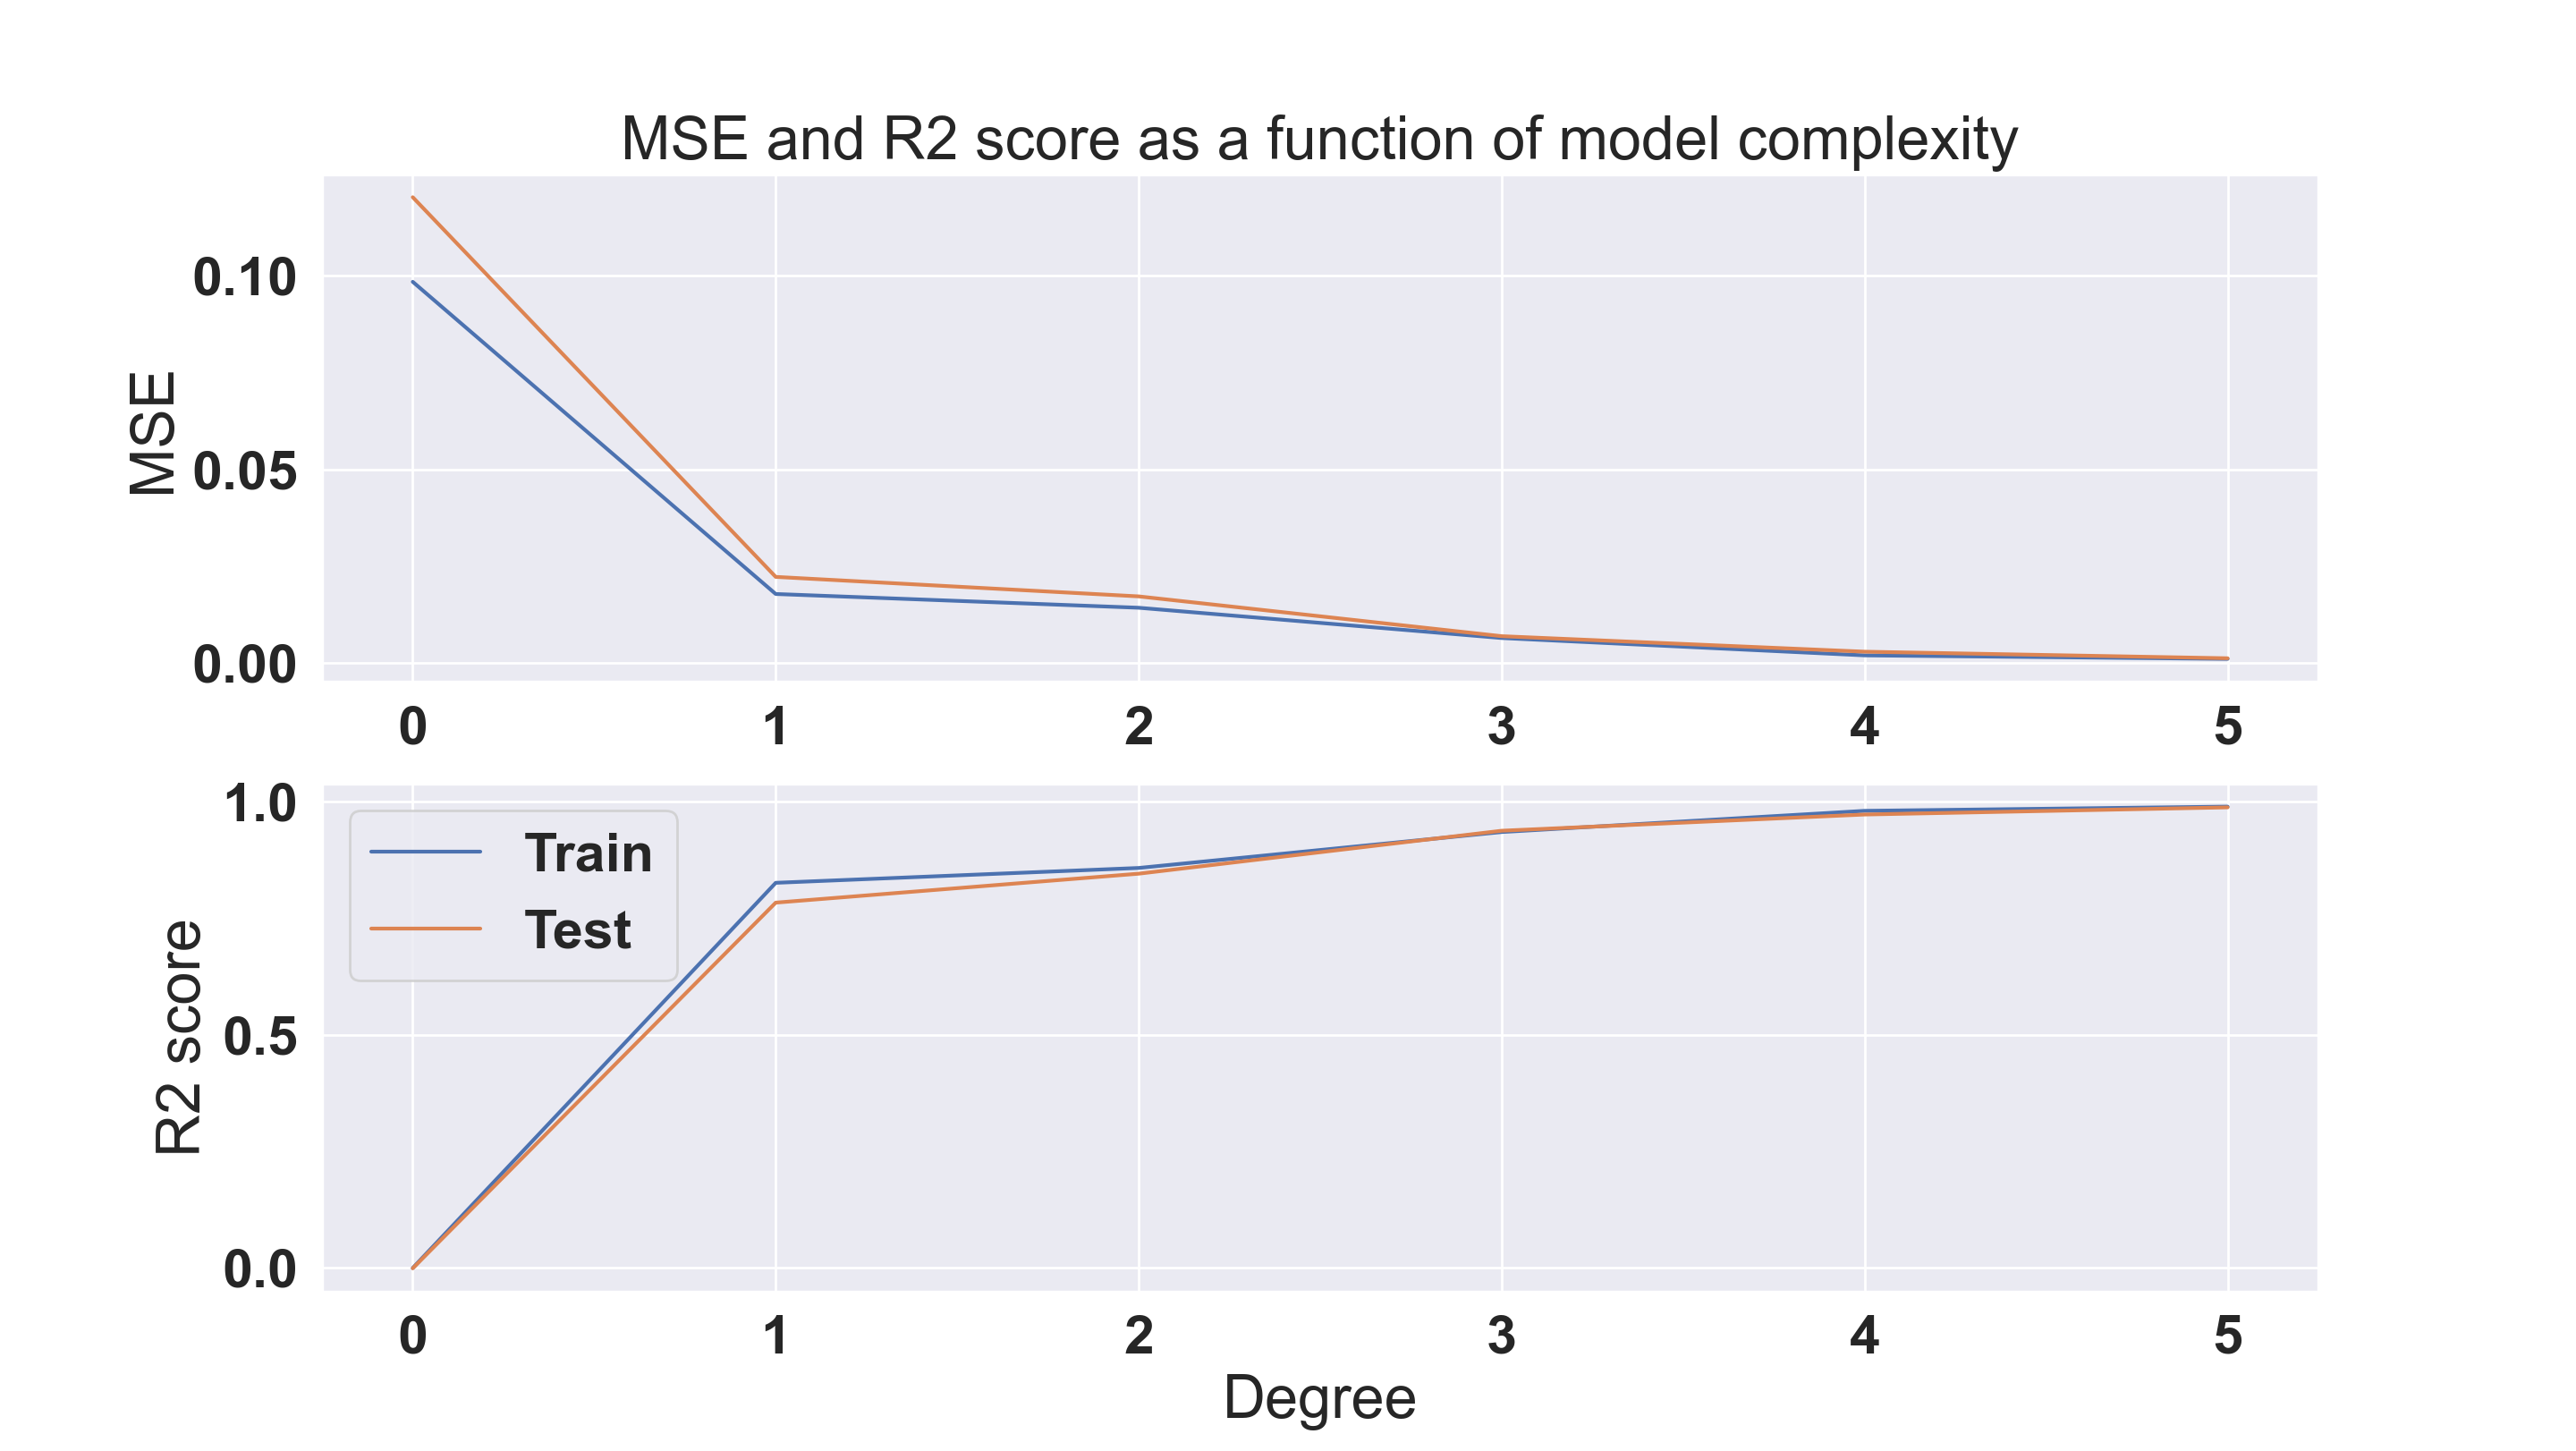
\includegraphics[width=0.5\textwidth]{Figure_3.png}
	\caption{Plot showing the MSE and R2 score for the franke function without noise. The regression method used was OLS}
	\label{MSE and R2 OLS}
\end{figure}
\noindent The next step was to include noise given by the normal distribution $\mathcal{N}(0,0.1)$. Figure \eqref{MSE and R2 OLS noise} shows
how the MSE and R2 score changes when noise is includet in to the data set.
\begin{figure}[h]
	\centering
	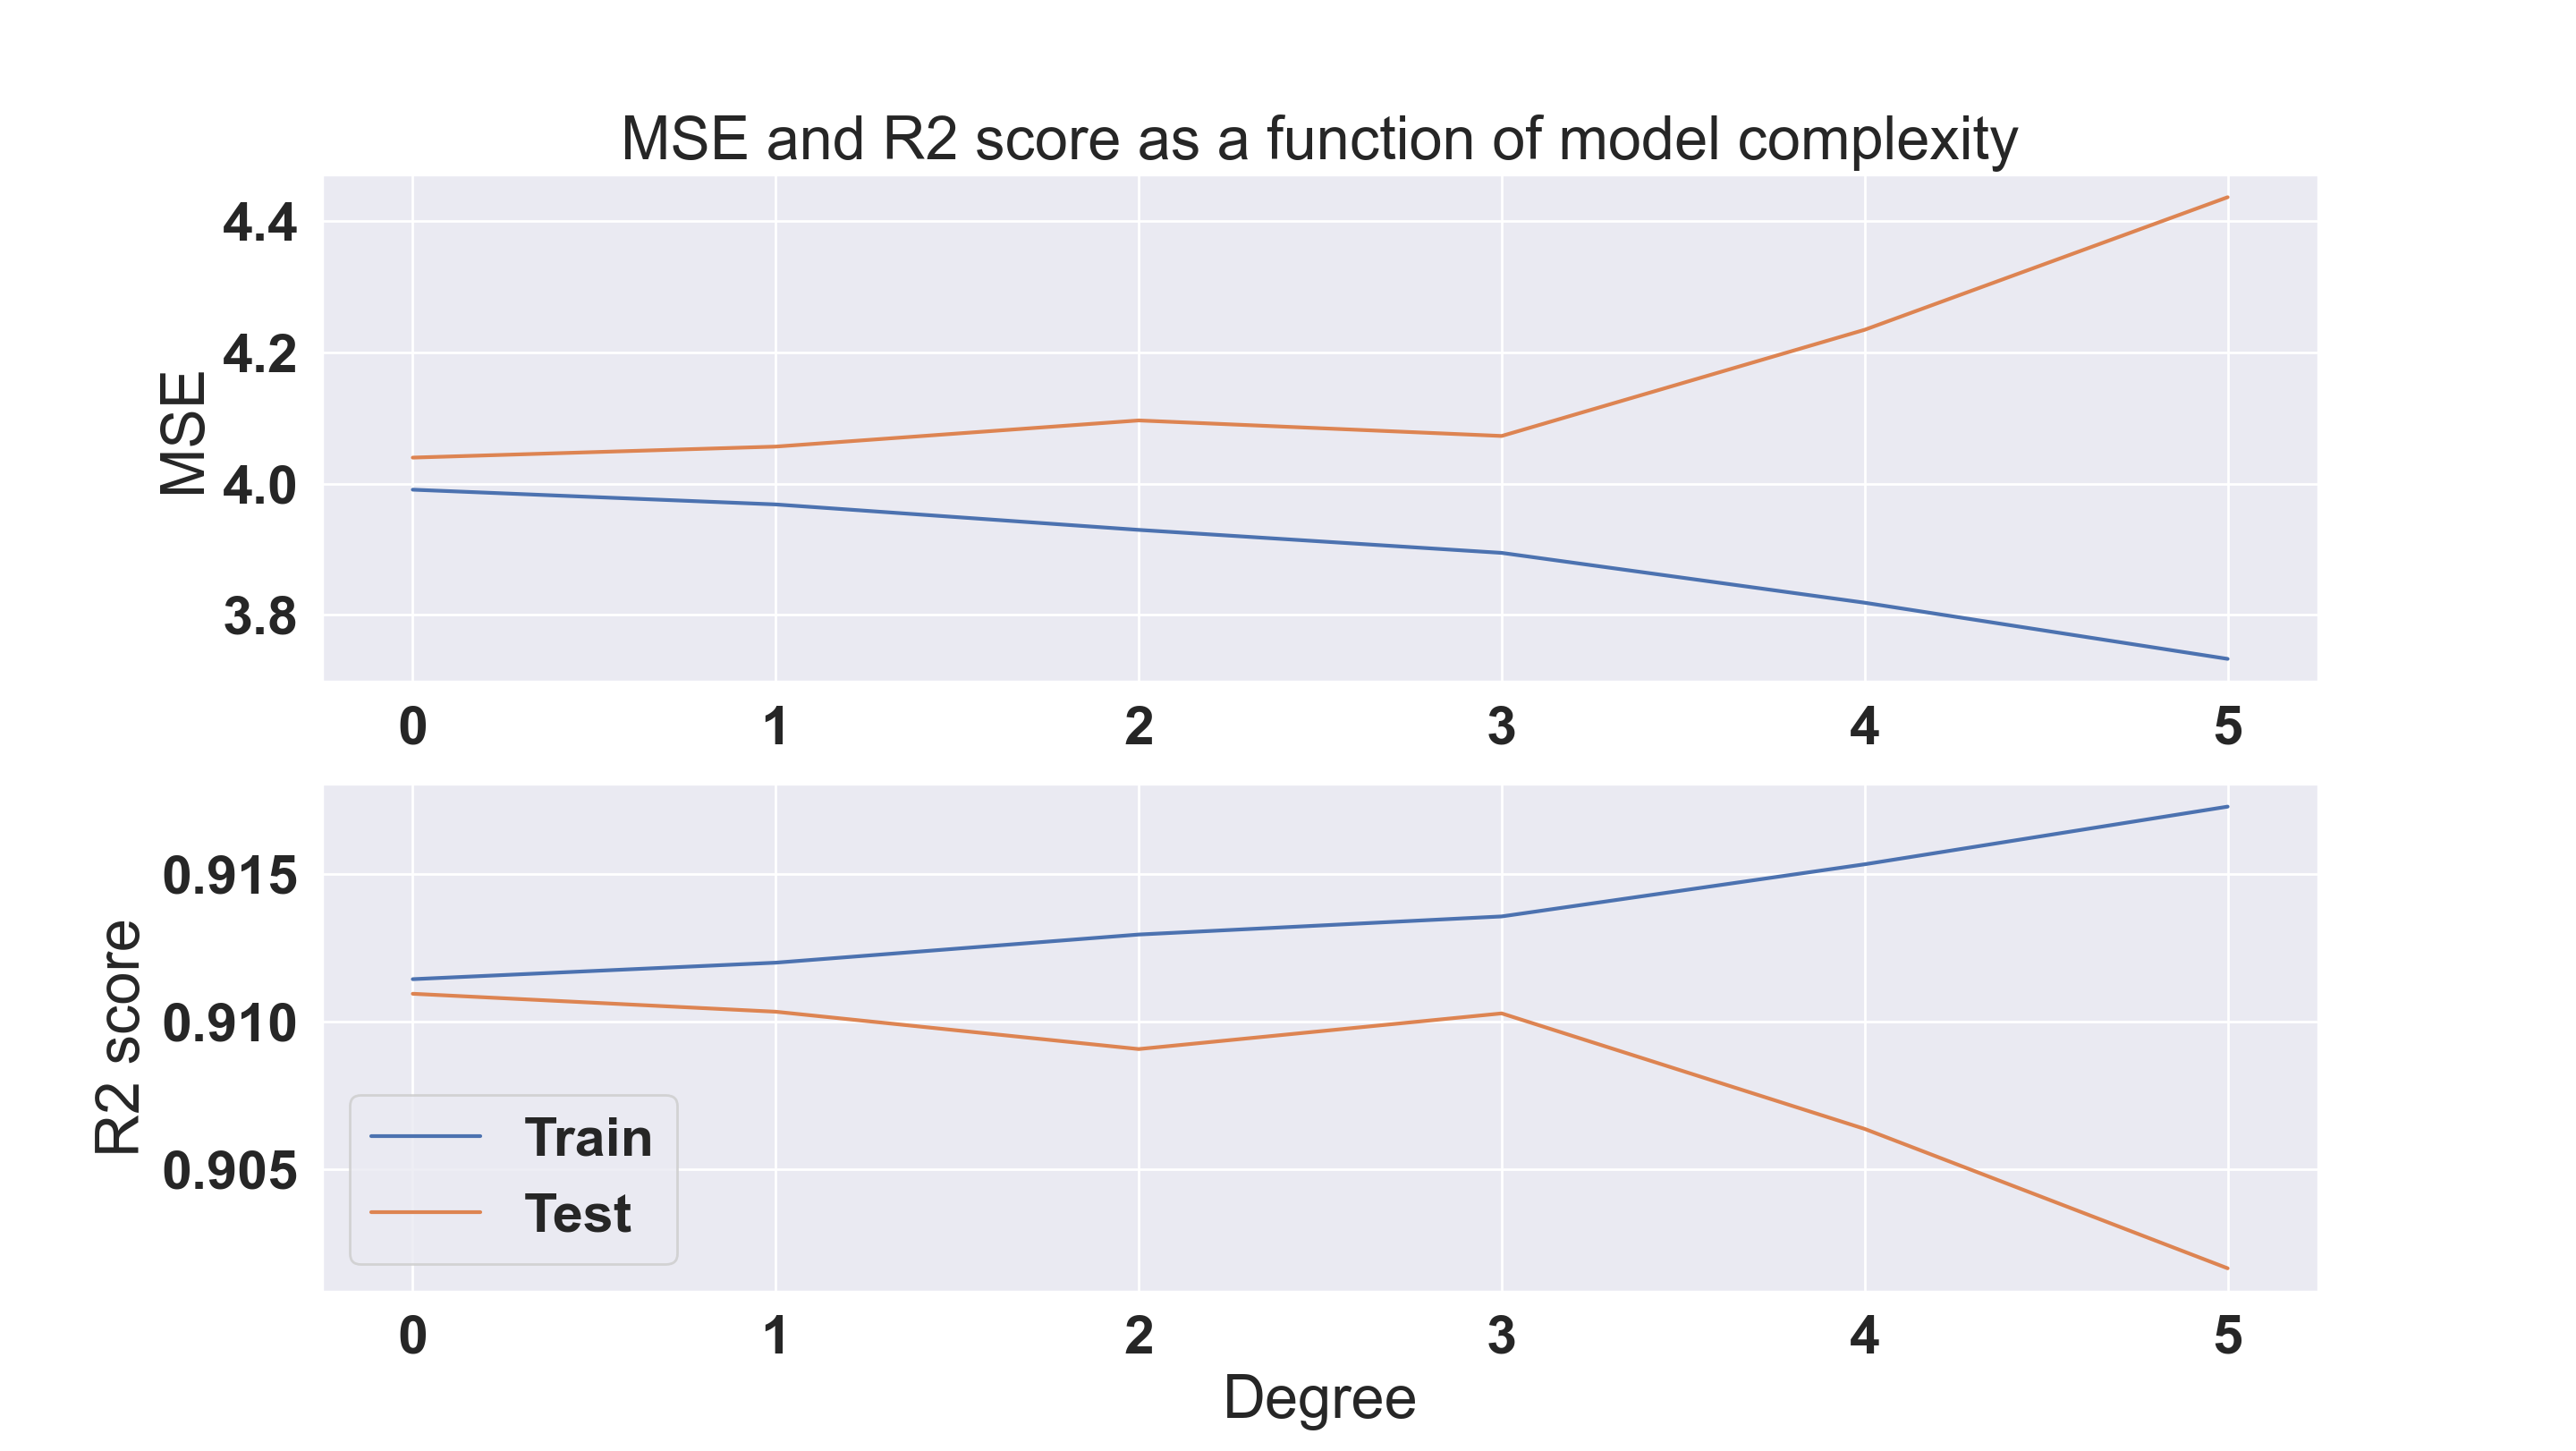
\includegraphics[width=0.5\textwidth]{Figure_4.png}
	\caption{Plot showing the MSE and R2 score for the franke function with noise $\mathcal{N}(0,0.1)$. The regression method used was OLS}
	\label{MSE and R2 OLS noise}
\end{figure}
\newline \newline
\textbf{Insert $\beta$ plott}
\newline \newline

\noindent For Ridge Regression on the franke function have we plotted a heatmap to show 
how the MSE changes with diffrent $\lambda$ values and complexities. A plot of
the heatmap for the training data is shown in figure \eqref{heatmap training ridge}
, and the heatmap for the test data is shown in figure \eqref{heatmap test ridge}.
\begin{figure}[h]
	\centering
	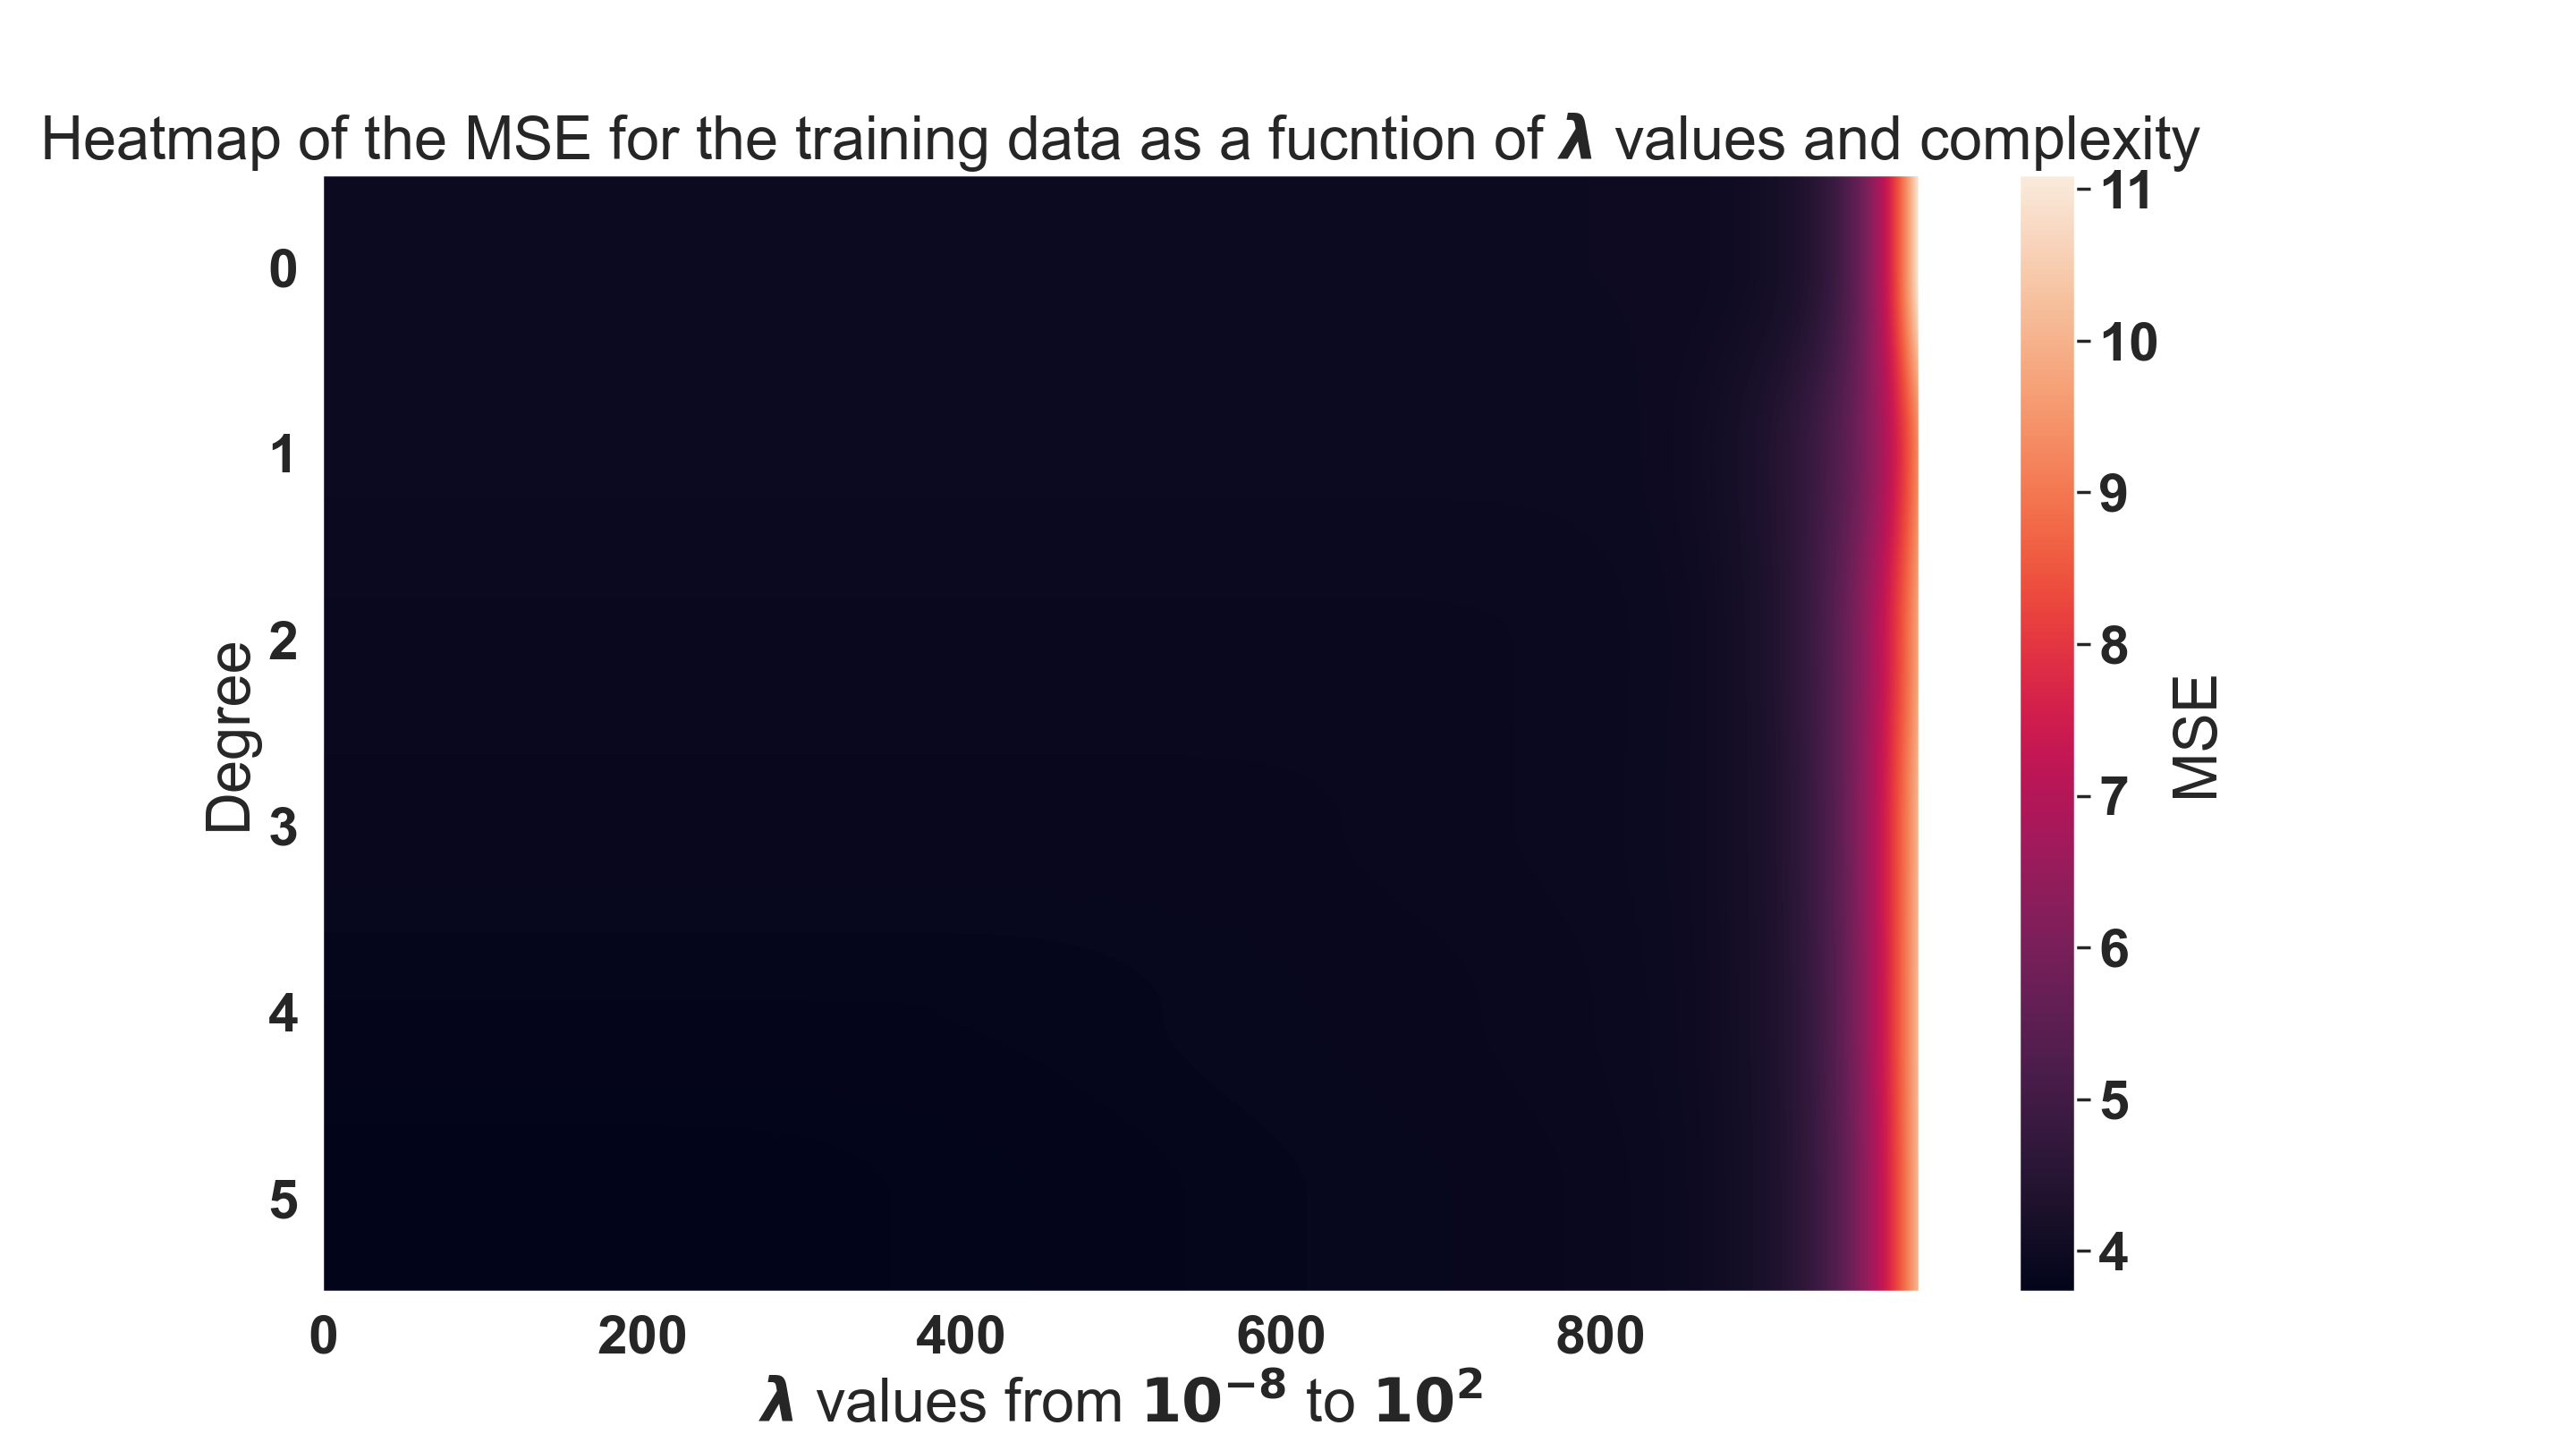
\includegraphics[width=0.5\textwidth]{Figure_8.png}
	\caption{A heatmap of the MSE for the training data, for different $\lambda$ values and complexities. The $\lambda$ values goes from $10^{-8}$ to $10^{2}$ }
	\label{heatmap training ridge}
\end{figure}
\begin{figure}[h]
	\centering
	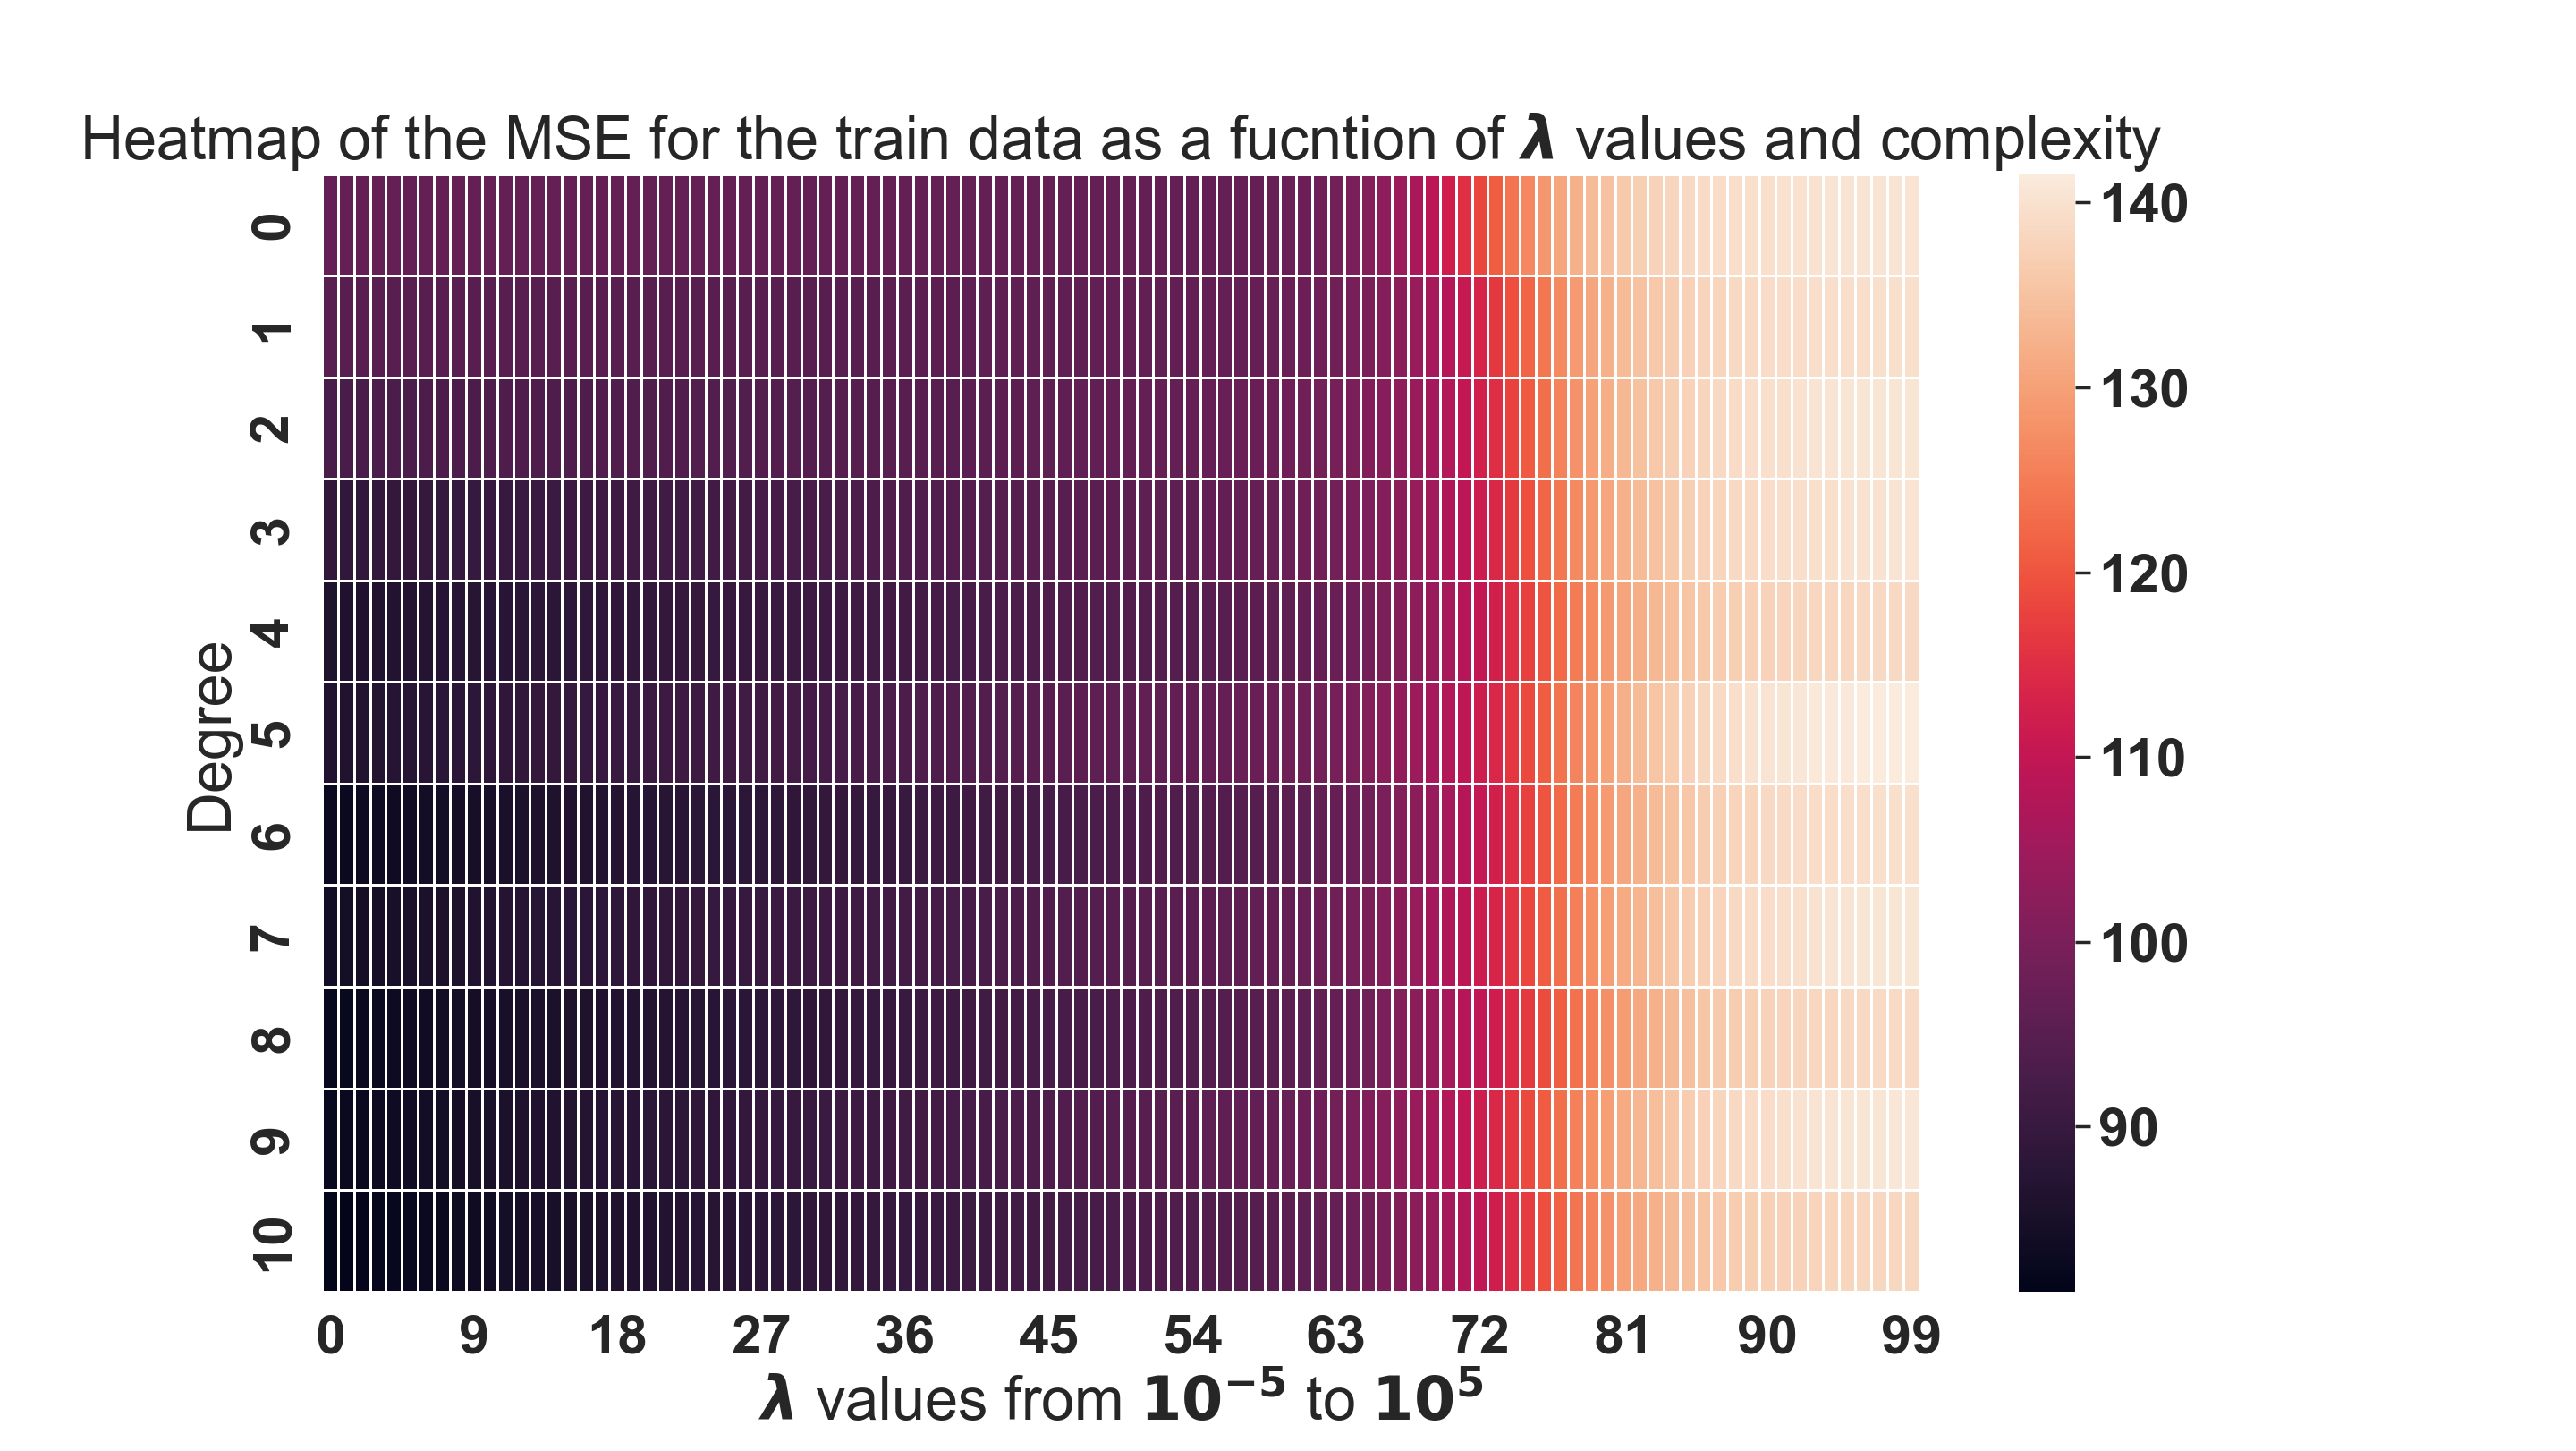
\includegraphics[width=0.5\textwidth]{Figure_7.png}
	\caption{A heatmap of the MSE for the testing data, for different $\lambda$ values and complexities. The $\lambda$ values goes from $10^{-5}$ to $10^{5}$}
	\label{heatmap test ridge}
\end{figure}
Lastly for Ridge regression we see what happens when $\lambda$ is put to zero.




\begin{figure}[h]
	\centering
	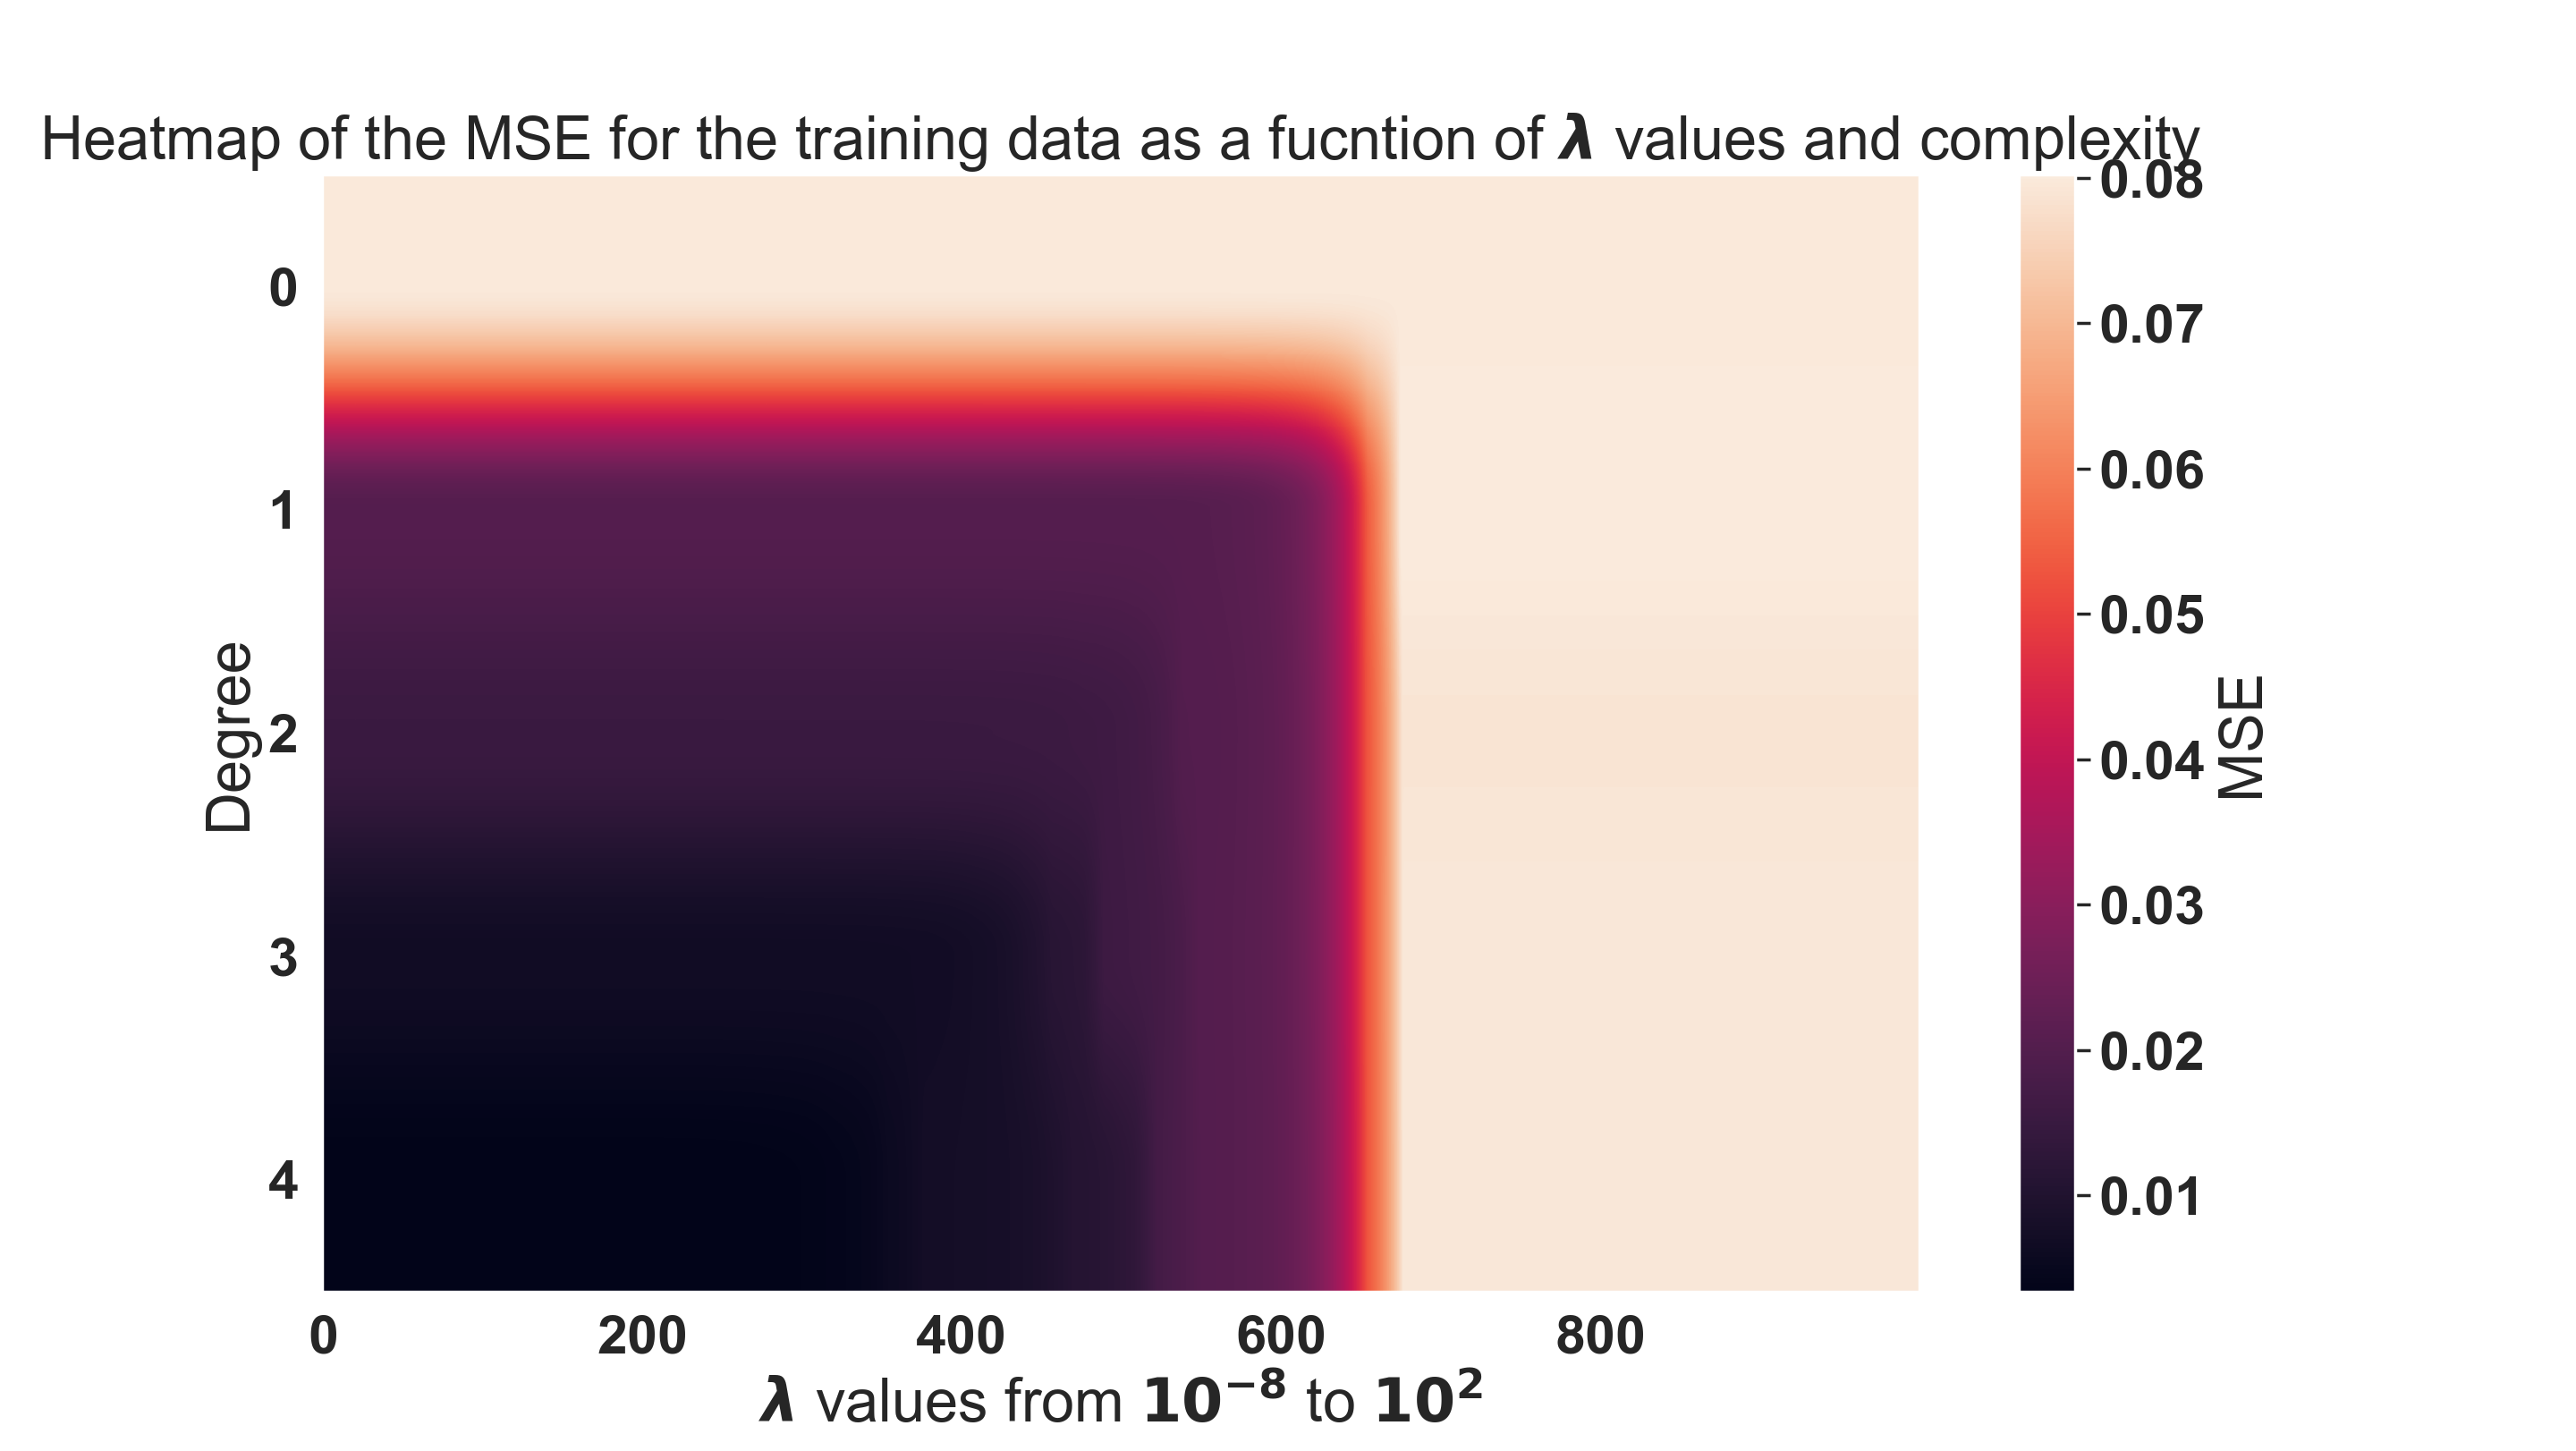
\includegraphics[width=0.5\textwidth]{Figure_9.png}
	\caption{A heatmap of the MSE for the training data, for different $\lambda$ values and complexities. The $\lambda$ values goes from $10^{-8}$ to $10^{2}$ }
	\label{heatmap training LASSO}
\end{figure}
\begin{figure}[h]
	\centering
	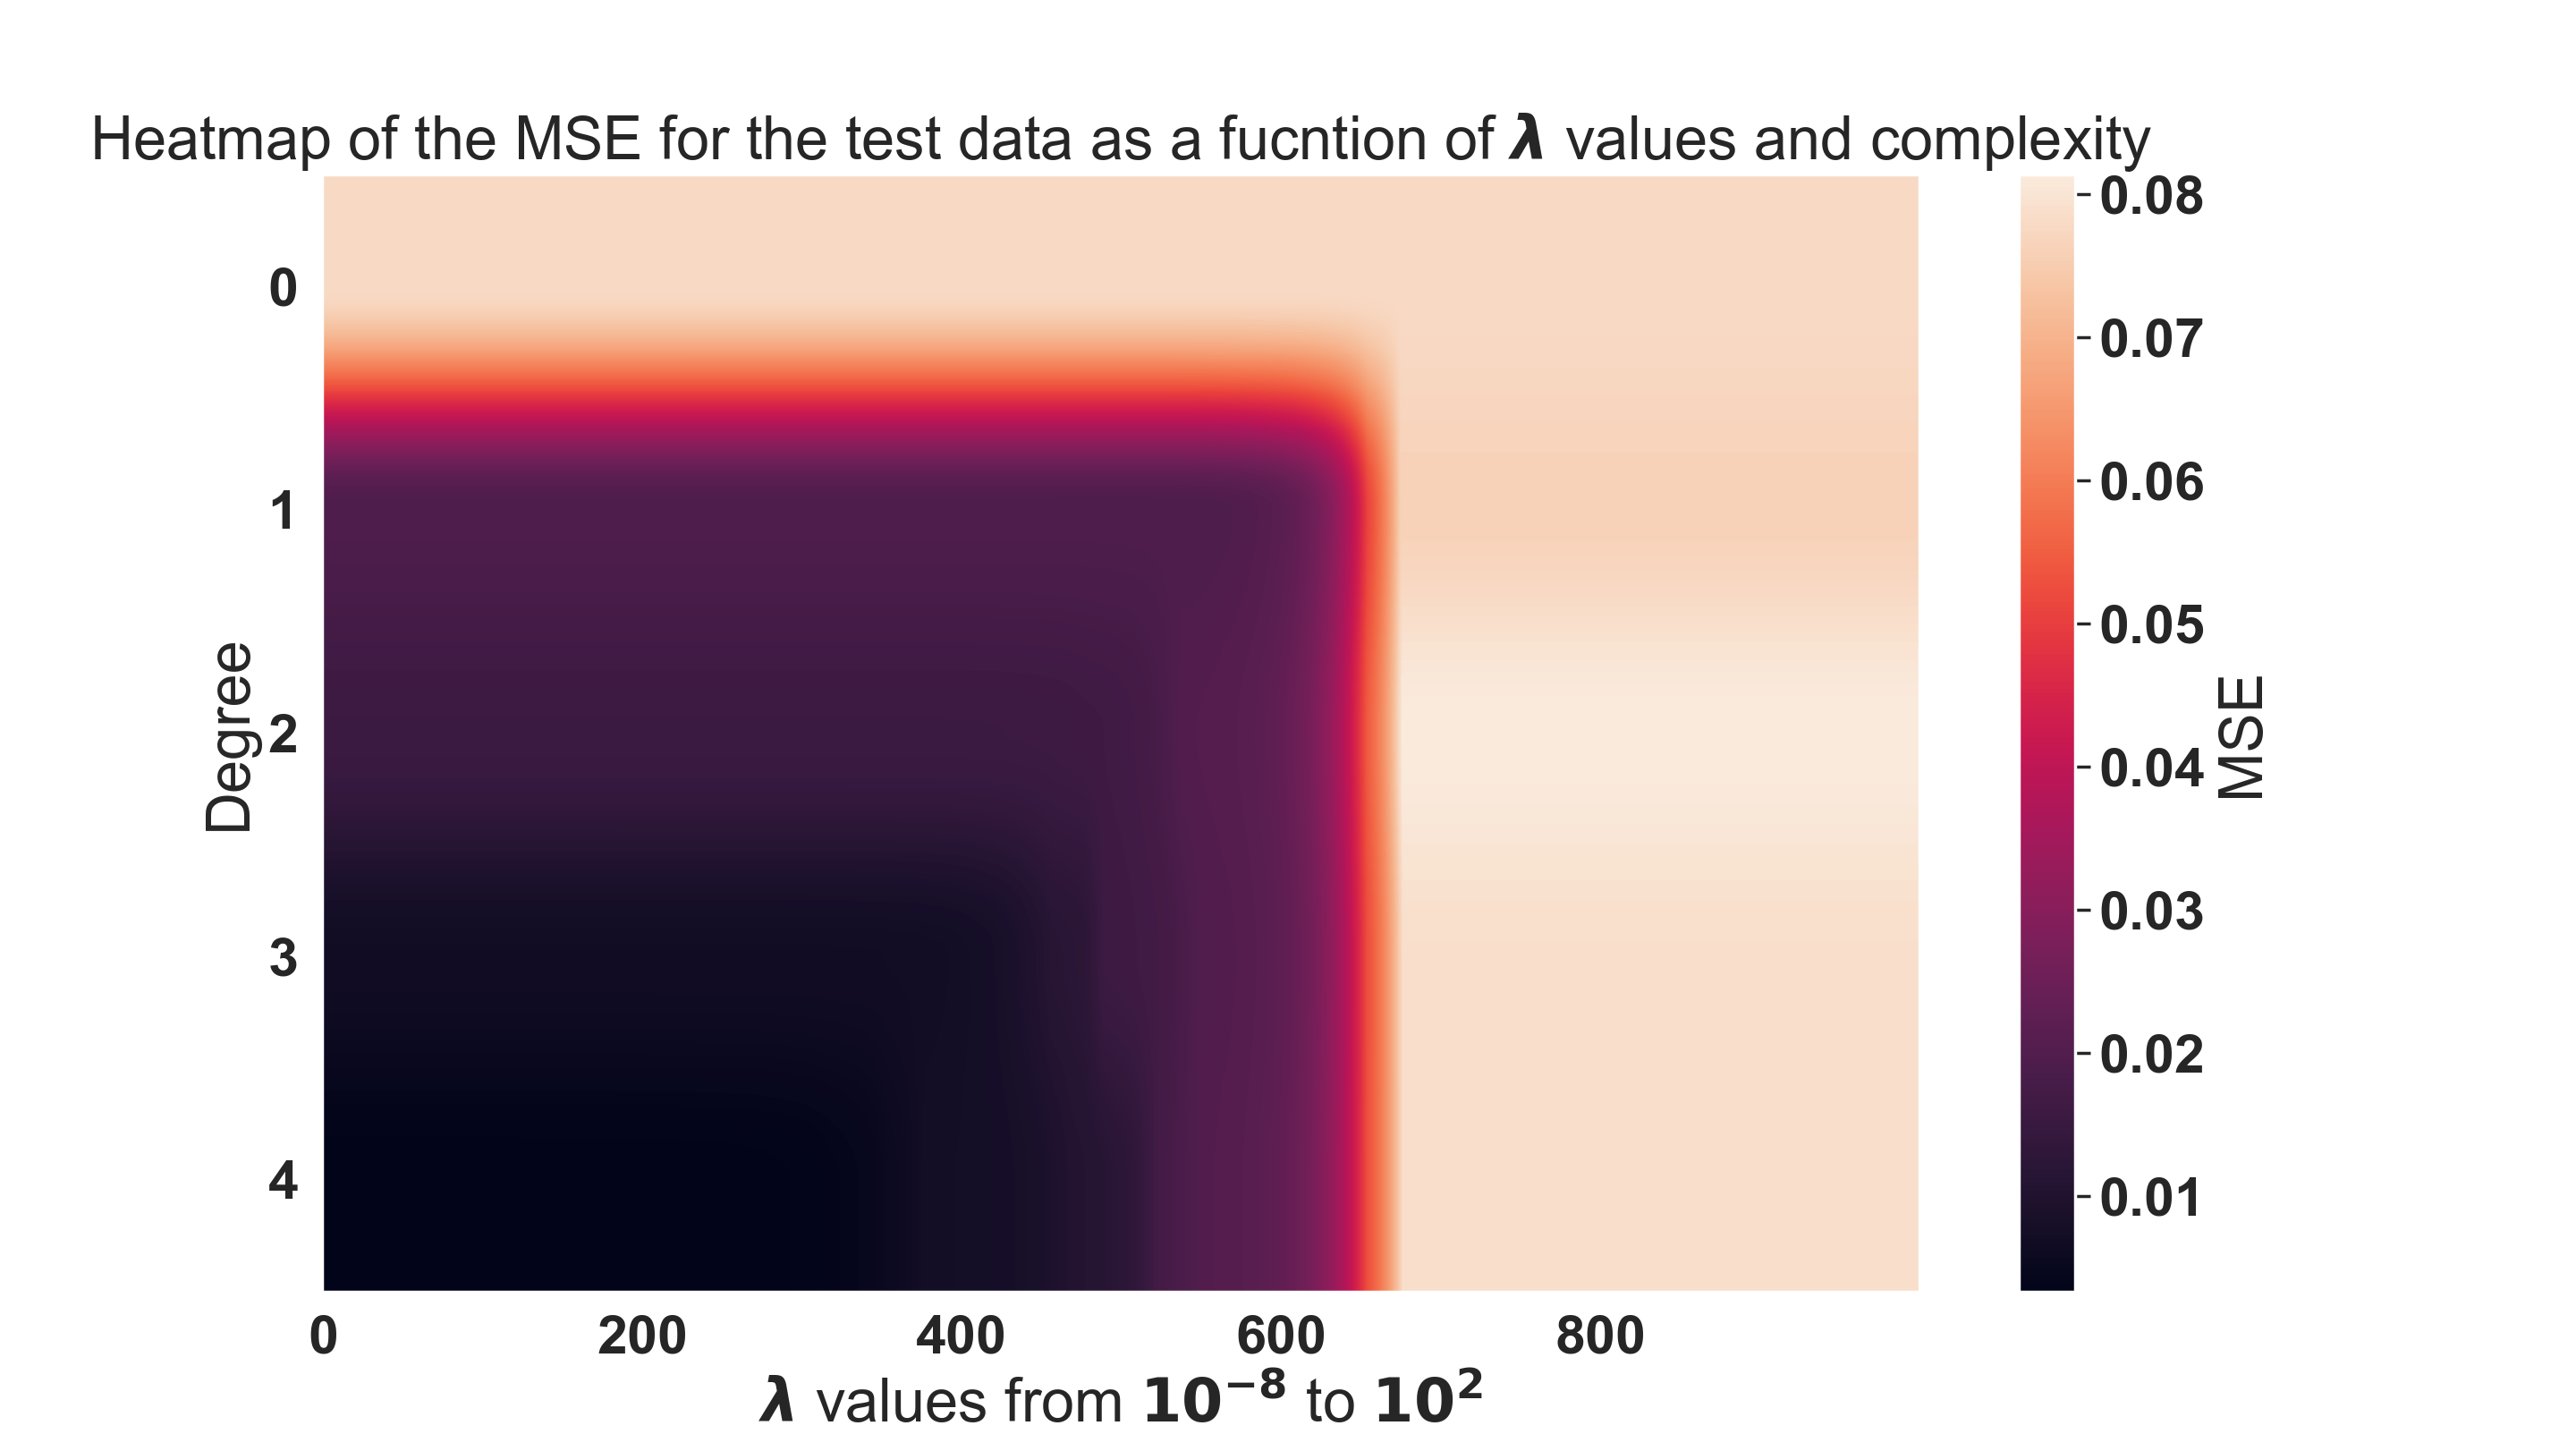
\includegraphics[width=0.5\textwidth]{Figure_10.png}
	\caption{A heatmap of the MSE for the testing data, for different $\lambda$ values and complexities. The $\lambda$ values goes from $10^{-5}$ to $10^{5}$}
	\label{heatmap test LASSO}
\end{figure}




\begin{figure*}[h]
	\centering
	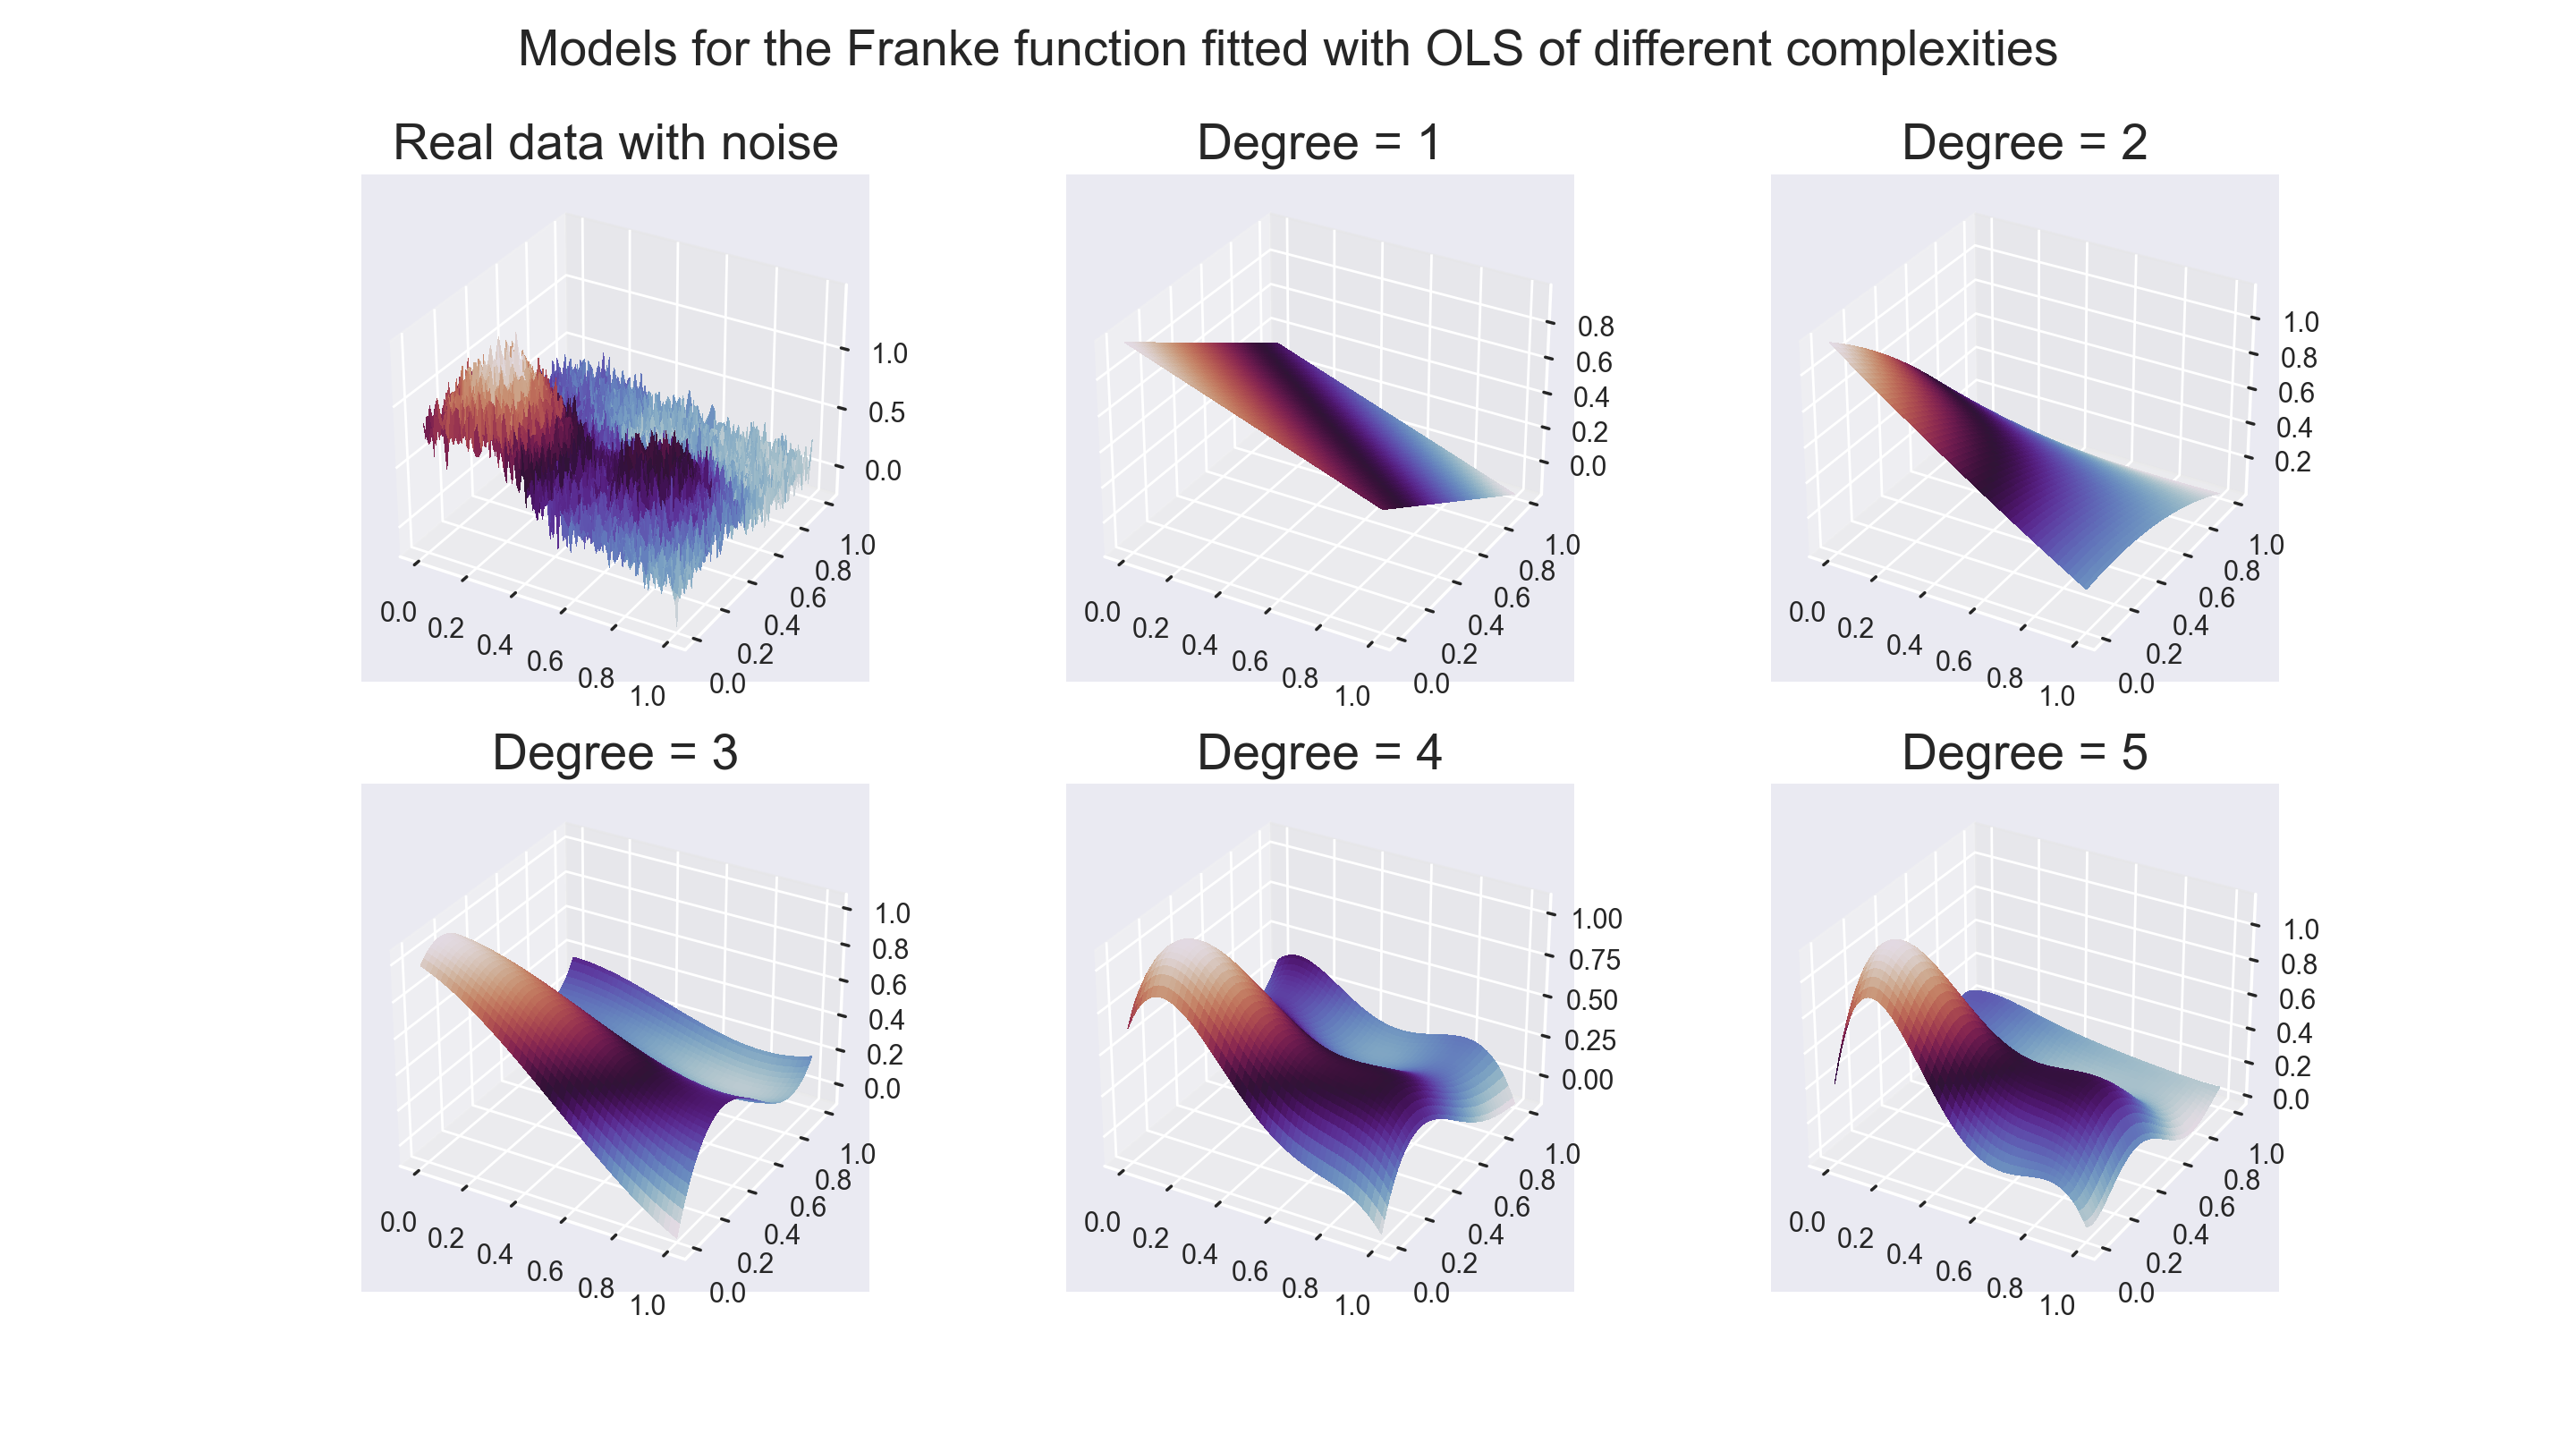
\includegraphics[width=\textwidth]{Figure_2.png}
	\caption{A plot showing how model with different complexities fit the franke function when OLS regession has been used.}
	\label{OLS figure}
\end{figure*}


\begin{figure*}[h]
	\centering
	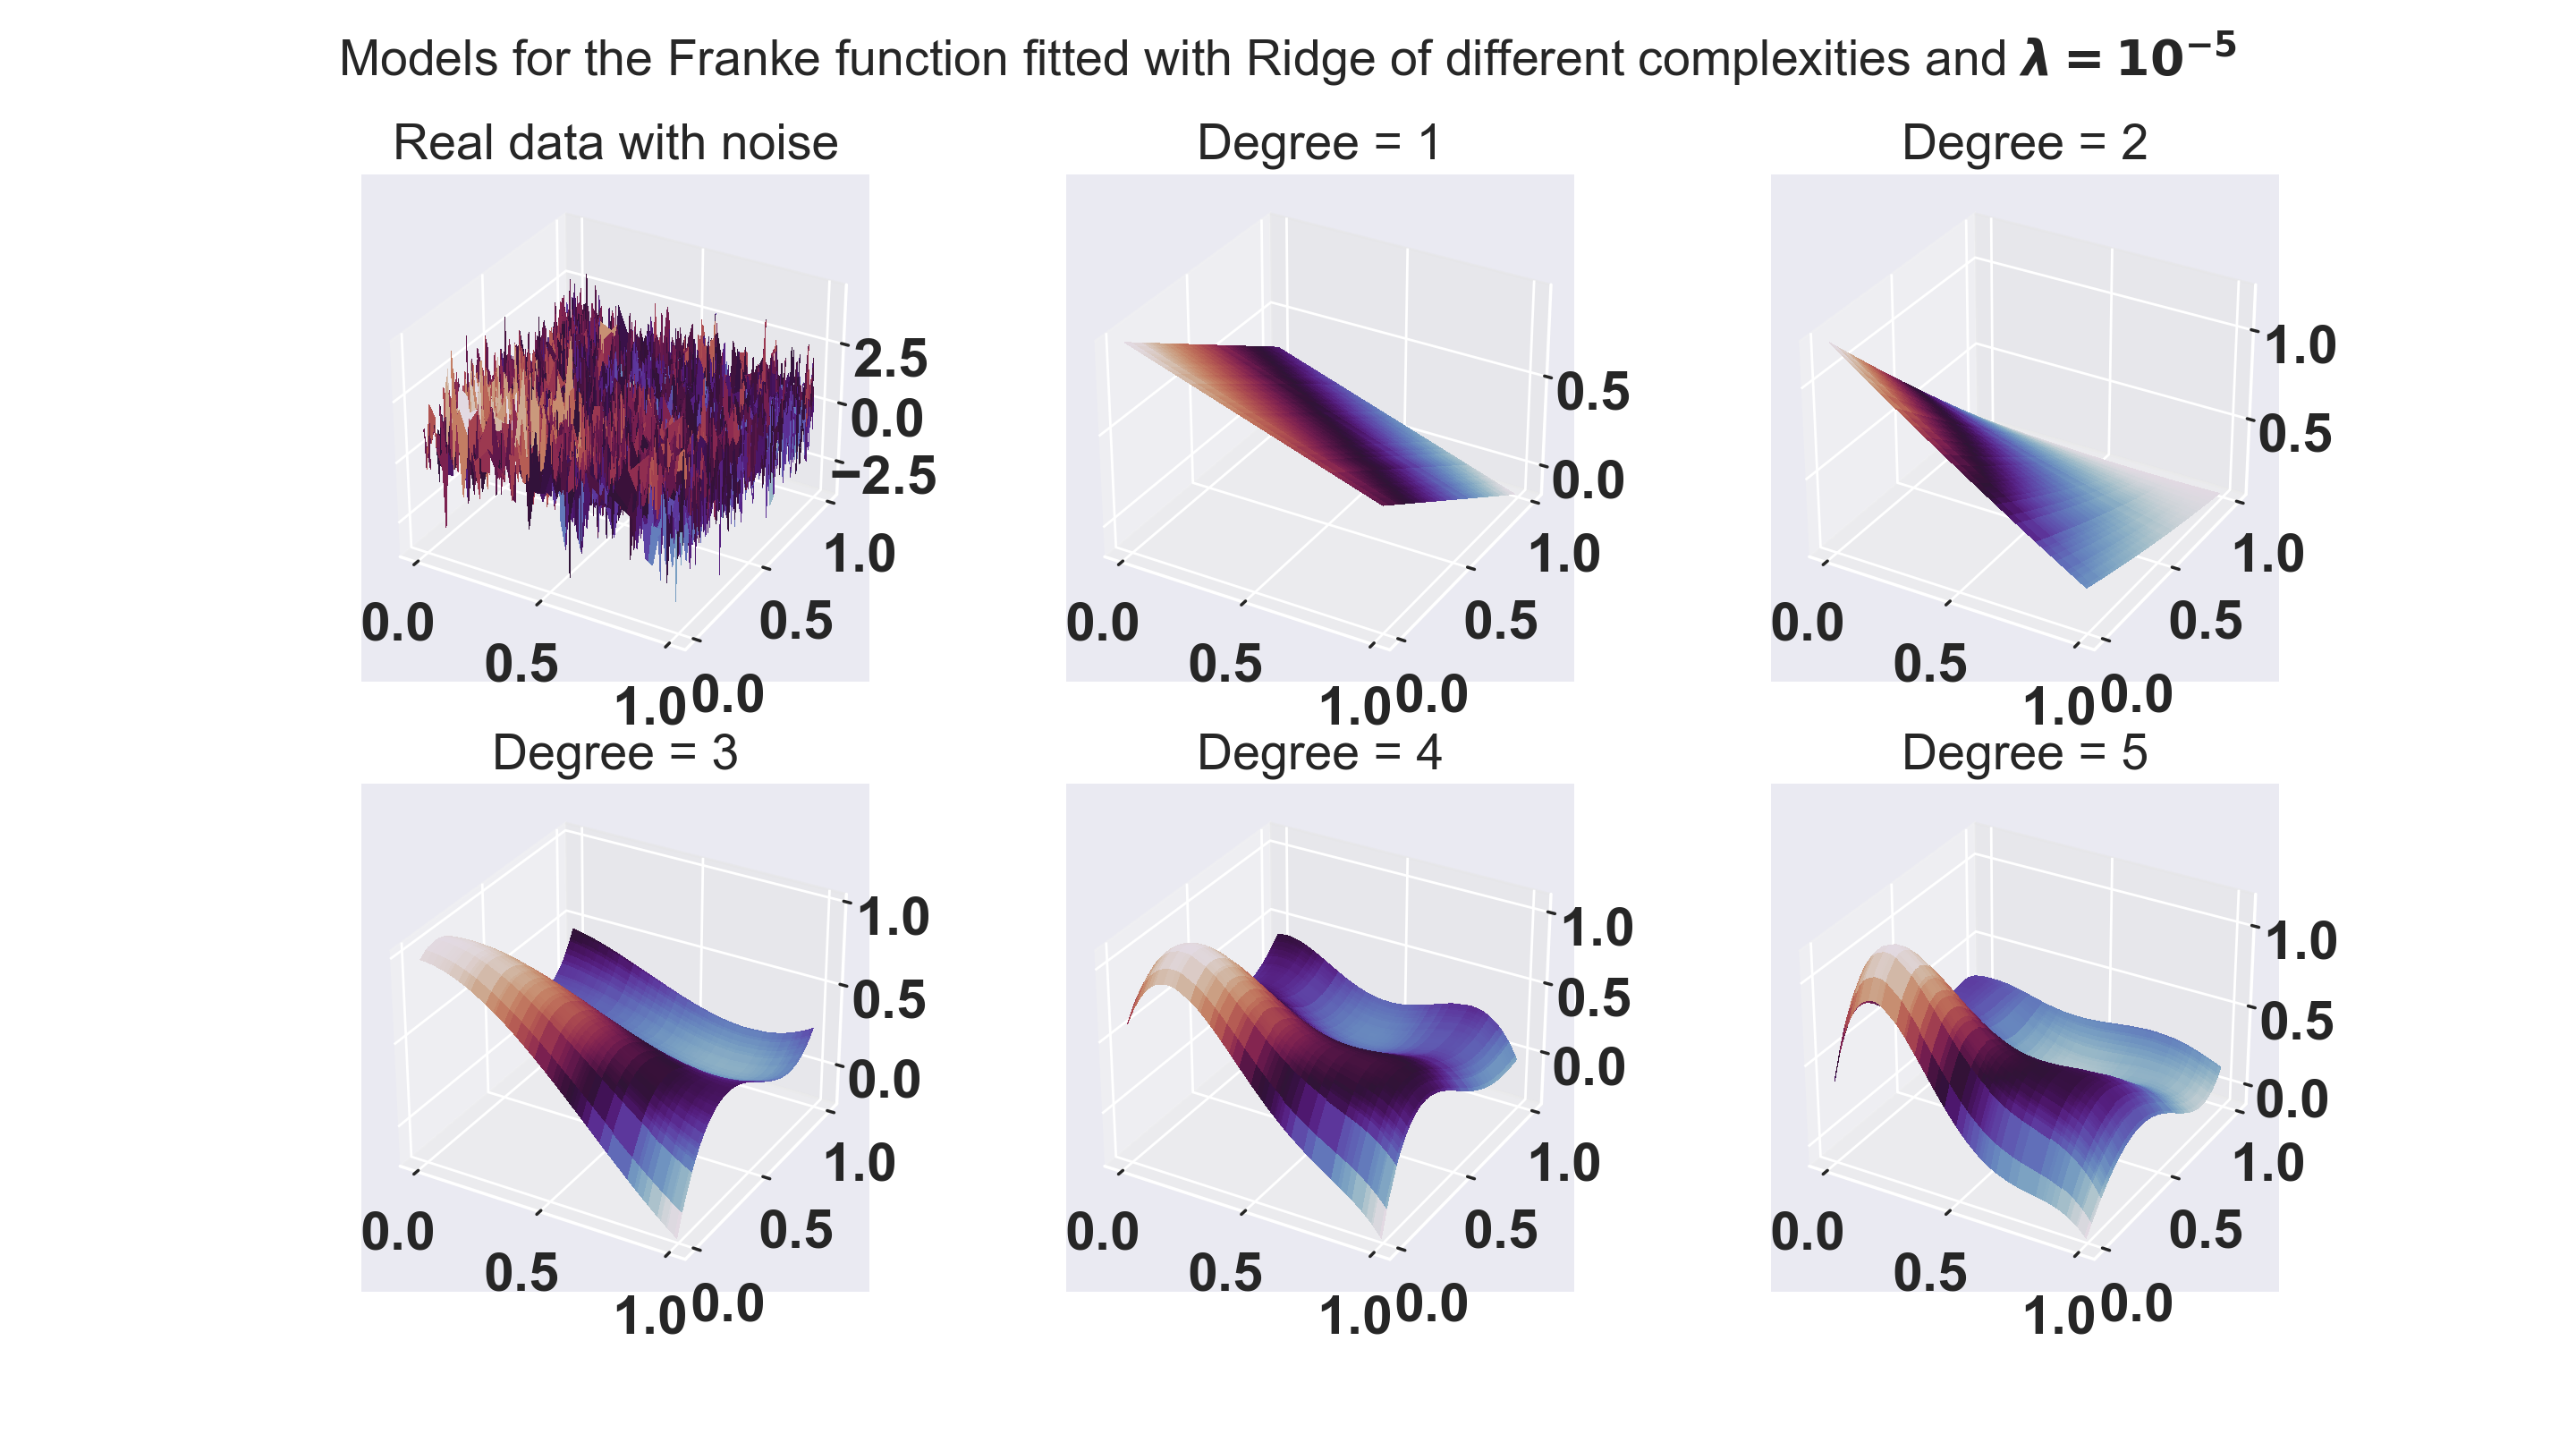
\includegraphics[width=\textwidth]{Figure_6.png}
	\caption{}
	\label{Ridge figure}
\end{figure*}

\begin{figure*}[h]
	\centering
	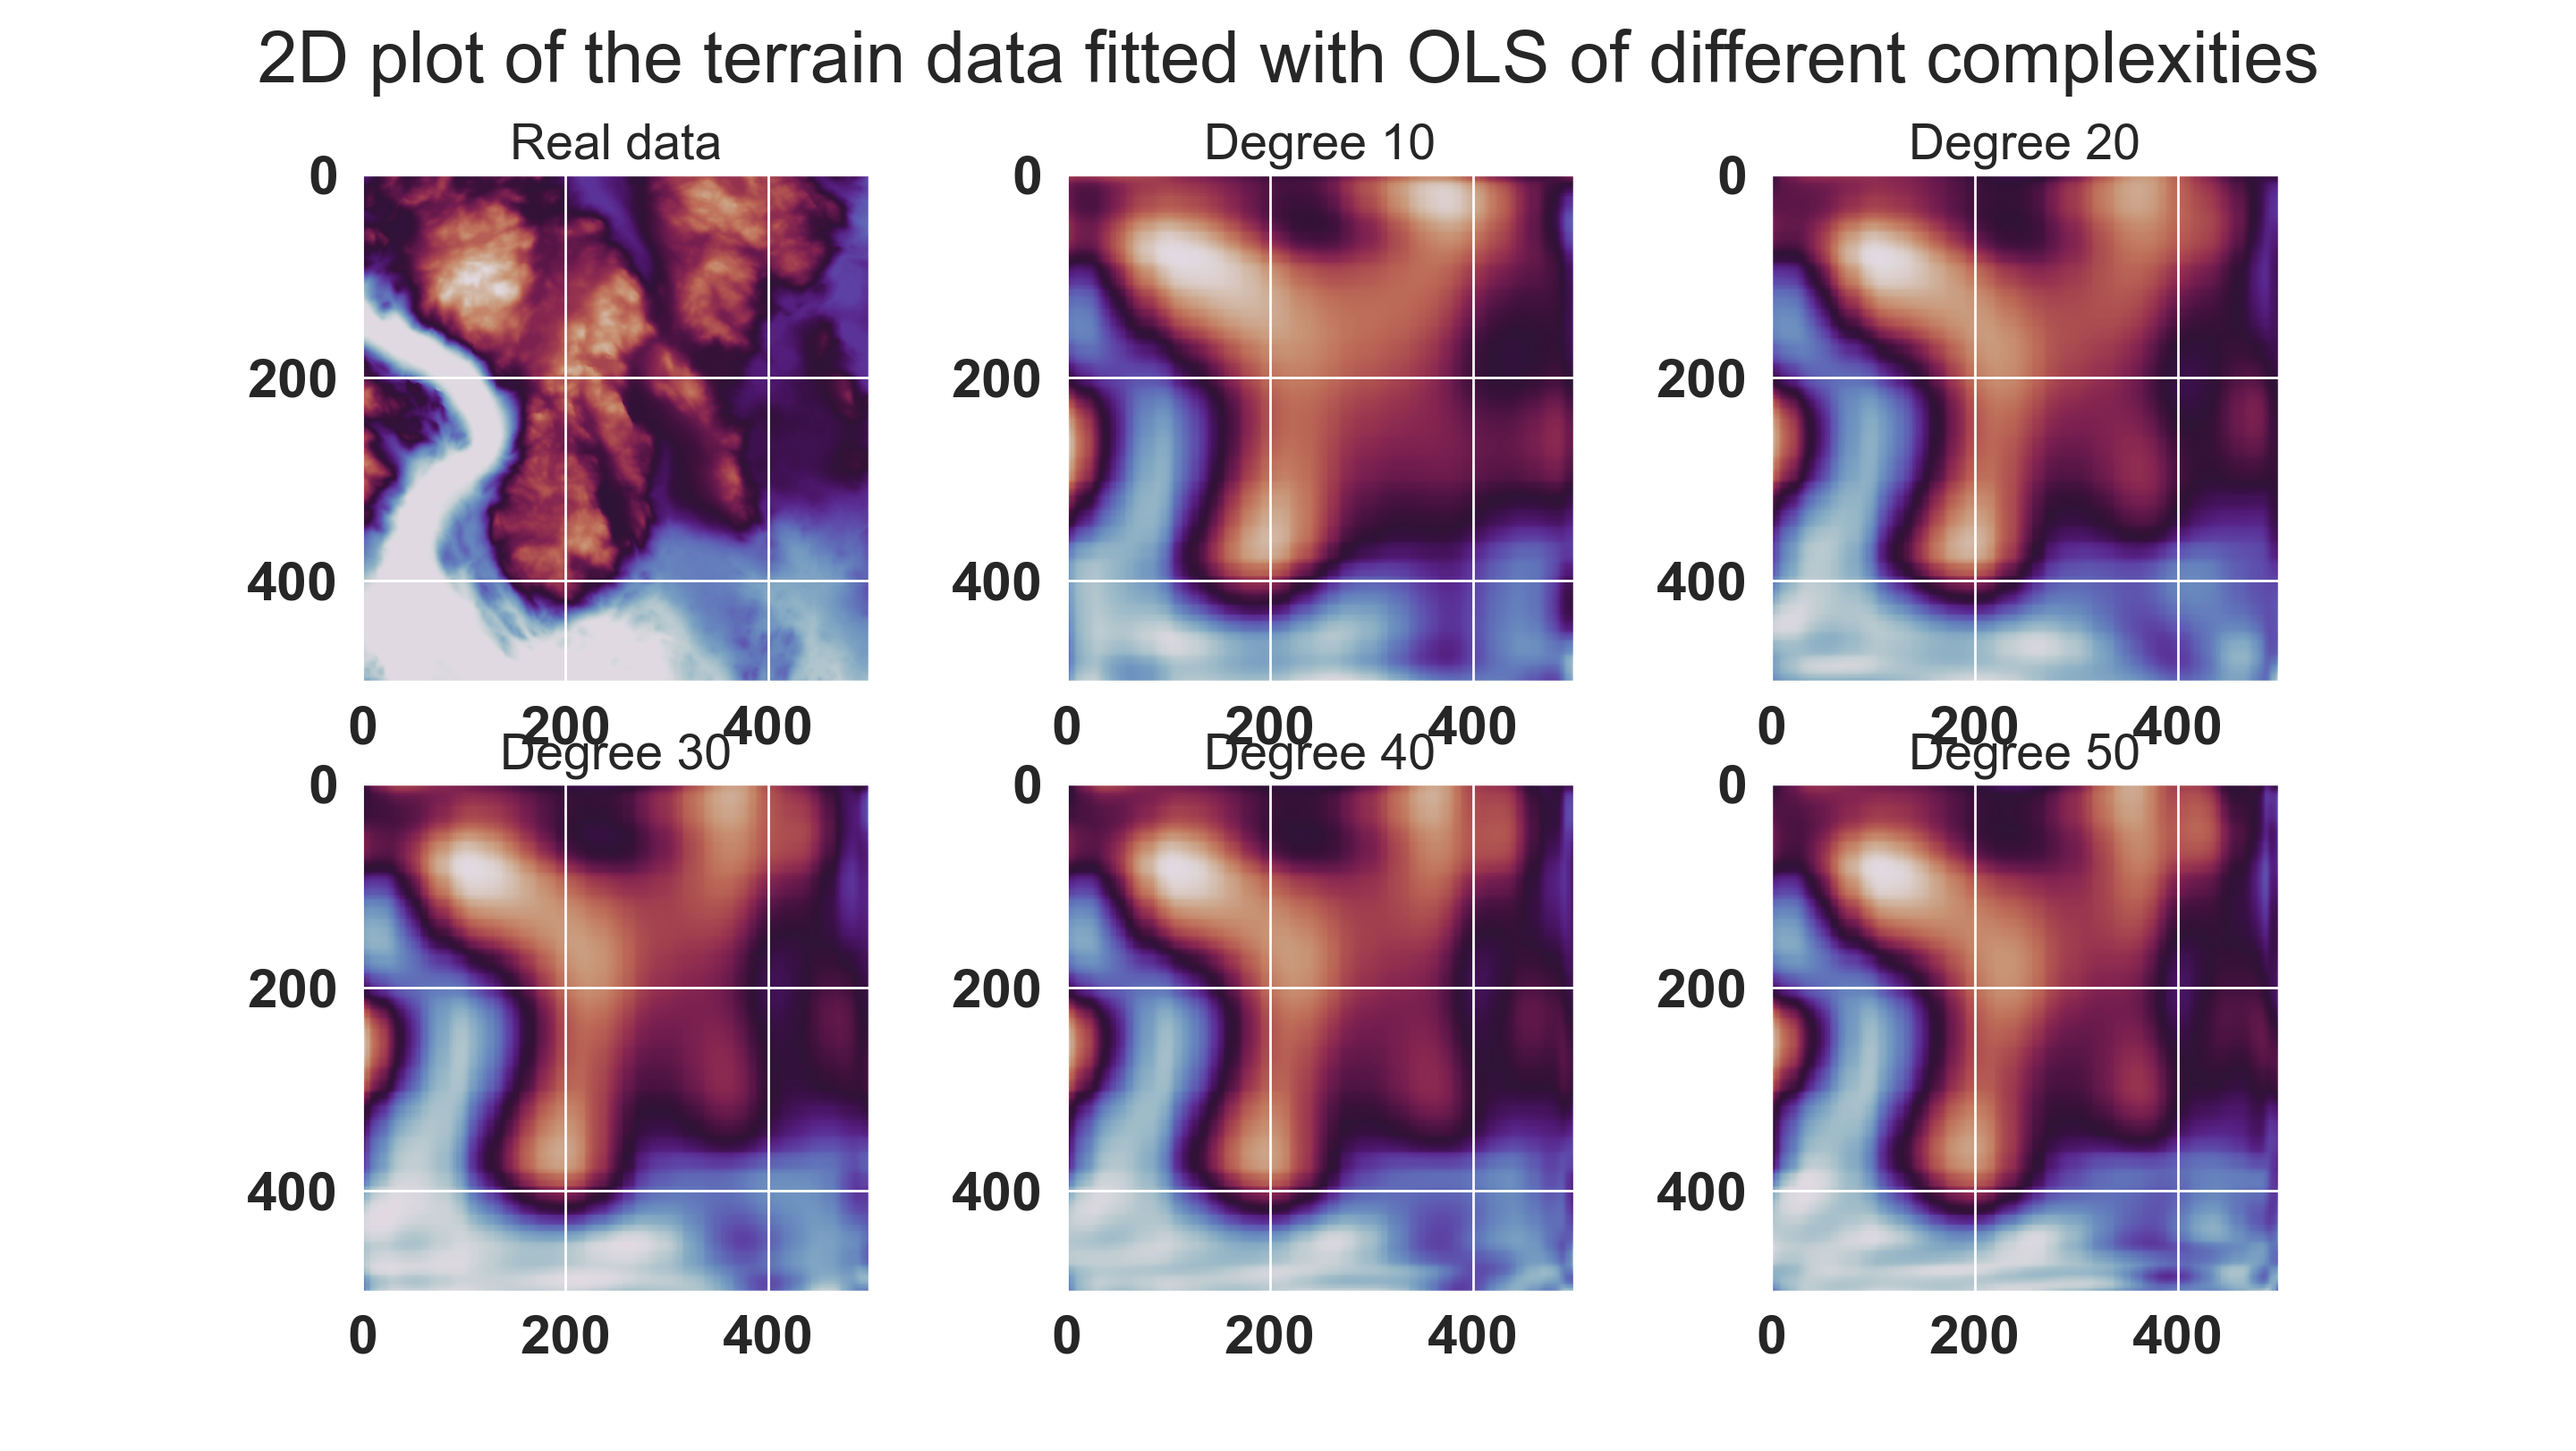
\includegraphics[width=\textwidth]{Figure_5.png}
	\caption{}
	\label{OLS figure terrain data}
\end{figure*}
\subsection{Results for terrain data}
